\subsection{Added value for the applicant's career and home institution}
This project represents a key advancement in my early scientific career, positioning me as the lead for integrating advanced research with translational clinical applications. As the responsible developer of GenomeSwift - the inaugural product from the \pmu - I am building a novel approach to translational research in medicine. This role will enhance my leadership skills to meet the expectations of the \pmu. 
Simultaneously, managing GenomeSwift's deployment in real-time, critical care settings will help me lay a foundation for innovative disease treatment methodologies.

This initiative will demonstrate \textbf{UZH}'s proficiency 
for creating and managing complex datasets, thereby becoming an essential asset for a broad range of rare disease, starting in metabolism, and planed to expand into immunology, endocrinology, and diabetology.

By spearheading the adoption of innovative omic analysis techniques, this project promises to markedly elevate both my professional growth and \textbf{UZH}'s influence in the realm of precision medicine.
Further details are provided in our whitepaper: 
\href{https://downgit.github.io/#/home?url=https://github.com/DylanLawless/precision_med_group/blob/main/whitepaper_1/whitepaper_1.1.pdf}{< link to github.com PDF download>}.

\subsection{Value analysis}

\subsubsection{Comparable benchmarks}
\label{sec:benchmarks}

The following studies are a subset of benchmarks that show the potential of precision medicine, particularly through genomic sequencing and multi-omic technologies, in diagnosing and managing rare and complex conditions. 
By implementing known methods, we can improve patient outcomes, enable targeted therapies, and potentially reduce healthcare costs through more accurate and faster diagnoses.
This integration promises not only to improve patient care but also to provide critical insights into the genetic basis of diseases, ultimately informing both treatment and prevention strategies.

The economic impact of critical care \citep{van2022hospital} reveals substantial costs per patient (systematic review: €1,101 to €91,951). In genomic insights for critically ill infants \citep{meng2017use}, molecular diagnoses affected medical management in over half the cases, utilizing critical trio exome sequencing. National scale multi-omics approaches for rare diseases \citep{lunke2023integrated} improved diagnostic yields to 54\% with integrated rapid whole-genome and transcriptomic data, significantly altering critical care management in 77\% of cases. A study on genomic lifespan associations in Iceland \citep{jensson2023actionable} identified actionable genotypes using whole-genome sequencing, which correlated with a decrease in median lifespan by three years. In the realm of neurodevelopmental disorders \citep{sanchis2023genome}, combined short-read and long-read sequencing identified causal variants in 36\% of the cases, highlighting the importance of long-read technology in resolving complex variants. Rapid whole-genome sequencing in the UAE \citep{abou2023rapid} demonstrated its utility with a quick turnaround, particularly noting its effectiveness in a Middle-Eastern population. Extensive genome sequencing for rare diseases \citep{wojcik2024genome} achieved a 29.3\% diagnostic yield, significantly identifying causative variants previously undetected by exome sequencing. Lastly, the UK and Ireland genomic diagnostics in paediatrics \citep{wright2023genomic} through the DDD study showed a 41\% diagnostic rate, emphasizing cost savings and targeted therapeutic potentials.

\subsection{Analysis results for \pmu}
Time series was performed using linear regression (for cost analysis) and Poisson regressions (for mortality  to extrapolate the expected outcomes from 2010-2030.
The actual cost and number of cases in for the past 12 years is accurately reported by BAG, however or estimate for future savings and benefit depend on the achievable benchmarks.
As our number update, we can build a more reliable model of what to expect over the next 10 years. 
The \pmu cost analysis overview is shown in figure 
\ref{fig:cost_analysis}.

\begin{figure}[h] \hspace*{0cm} 
\begin{center}
	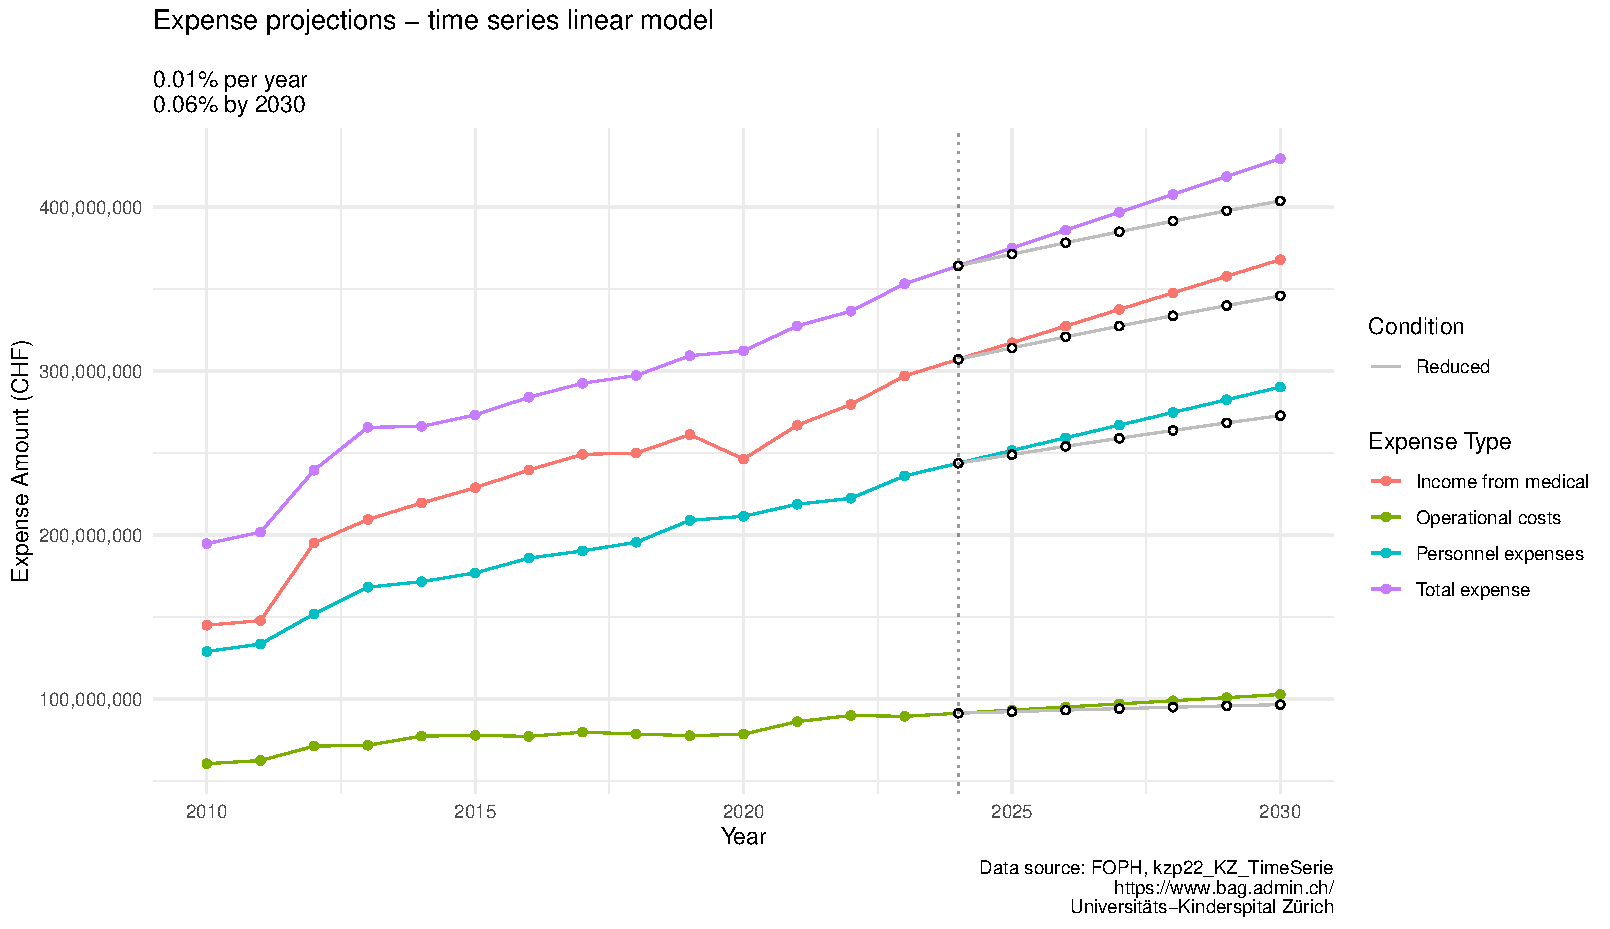
\includegraphics[width=0.90\textwidth]{../../stats/foph_key_stats/output/p_cost}
	\caption{Projections for Kispi with a \pmu (2010-2030). Federal statistics from Bundesamt für Gesundheit (BAG, Federal office for public health) were modelled and projected to 2030. A modest benefit effect size was applied. 
	In the most similar application to our \pmu; 
	\citet{lunke2023integrated} 
	showed a 54\% diagnostic yield and an altered critical care management in 77\% of diagnosed cases.
	We estimated modest 1\% increase in actualised savings per year after successful implementation starting in 2024.}
	\label{fig:cost_analysis}
\end{center}
\end{figure}

A more accurate demonstration of the \pmu can be seen with a specific disease example using sepsis.
Sepsis was specifically modelled using federal statistics from Bundesamt für Gesundheit (BAG, Federal office for public health) from 2010-2022 as shown in 
\textbf{figure
% \ref{fig:p_cases_sepsis_uni_yearly},
\ref{fig:p_cases_sepsis_kispi_yearly_forecast}}.
%\ref{fig:p_cases_per_indicator_kispi_2022}}.
% First we get a global picture of sepsis in University hospitals in  \textbf{figure \ref{fig:p_cases_sepsis_uni_yearly}}.  This illustrates the total number of sepsis in adult and paediatric settings across the country.
The forecast model, from 2010-2030, shows the number of deaths due to sepsis in \kispi (\textbf{Figure \ref{fig:p_cases_sepsis_kispi_yearly_forecast}}).
The predicted number of preventable deaths is based on comparable benchmarks listed in section 
\textbf{\ref{sec:benchmarks}}
which have demonstrated clear cost-saving potential through precise diagnostics and targeted therapy.
For rare diseases, approximately 40\% of probands received a genetic diagnosis 
\citep{wright2023genomic, wojcik2024genome}
and altered critical care management in 77\% of diagnosed cases \citep{lunke2023integrated}.
A well-managed work-flow can result in rapid whole-genome sequencing with a turnaround of 37 hours on average
 \citep{abou2023rapid}.
Based on such values, the forecast  projected into 2030 shows the yearly cases of sepsis.
Black and red values show the expected number of deaths with and without  precise diagnostics and targeted therapy, respectively. 

%\begin{figure}[h] \hspace*{0cm} 
%\begin{center}
%	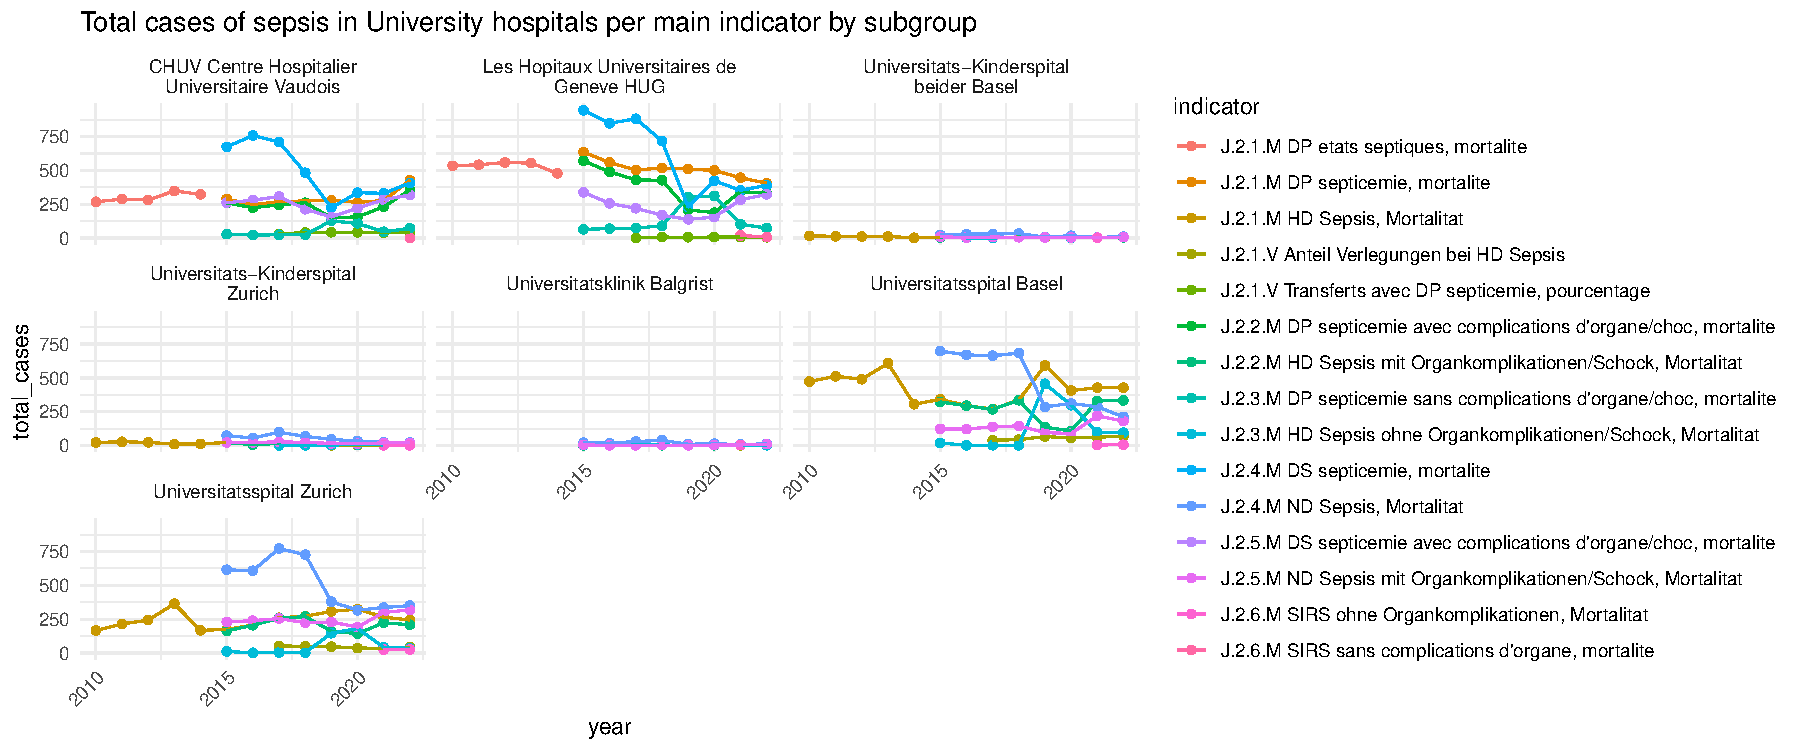
\includegraphics[width=1\textwidth]{../../stats/foph_key_stats/output/p_cases_sepsis_uni_yearly}
%	\caption{Yearly deaths due to sepsis at University hospitals across Switzerland.
%	This data is based on statistics reported by Bundesamt für Gesundheit (BAG), 
%	\url{https://www.bag.admin.ch/} for years 2010-2022. 
%		DP: Diagnostic procedure.
%HD: Primary diagnosis.
%ND: Secondary diagnosis.}
%	\label{fig:p_cases_sepsis_uni_yearly}
%\end{center}
%\end{figure}

\begin{figure}[h] \hspace*{0cm} 
\begin{center}
	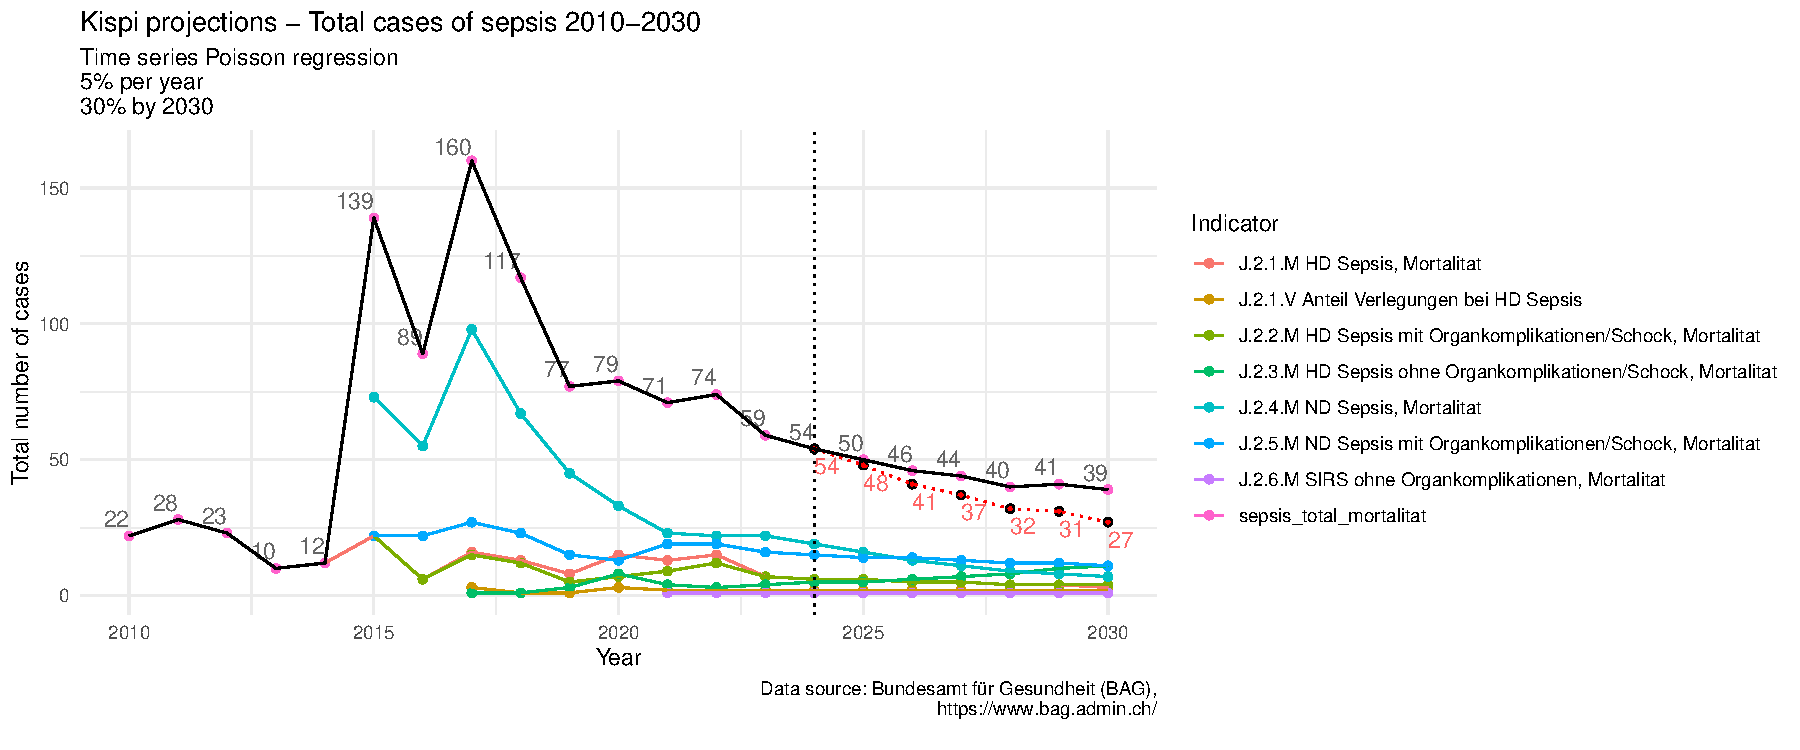
\includegraphics[width=1\textwidth]{../../stats/foph_key_stats/output/p_cases_sepsis_kispi_yearly_forecast}
	\caption{Yearly deaths due to sepsis at \kispi.
	This data is based on statistics reported by Bundesamt für Gesundheit (BAG), 
	\url{https://www.bag.admin.ch/} for years 2010-2022. 
	Time series was performed using Poisson regression to extrapulate the expected outcomes from 2010-2030.
	Predictions for the cost and number of cases were generated in section 
	\ref{sec:benchmarks}.	
	DP: Diagnostic procedure.
HD: Primary diagnosis.
ND: Secondary diagnosis.}
	\label{fig:p_cases_sepsis_kispi_yearly_forecast}
\end{center}
\end{figure}

To put the work of the \pmu in perspective, we look at the total number case statistics for \kispi.
We see a total number of all cases indicators in 2022 of \textbf{10'261}.
The subgroup indicator for ``J.2 sepsis'' shows \textbf{74} cases in 2022.
%\textbf{Figure \ref{fig:p_cases_per_indicator_kispi_2022}}  shows the the indicators through A1-Z4, many of which are similarly affected by the advances in precision medicine and are thus potential future prospects.

%\begin{figure}[h] \hspace*{0cm} 
%\begin{center}
%	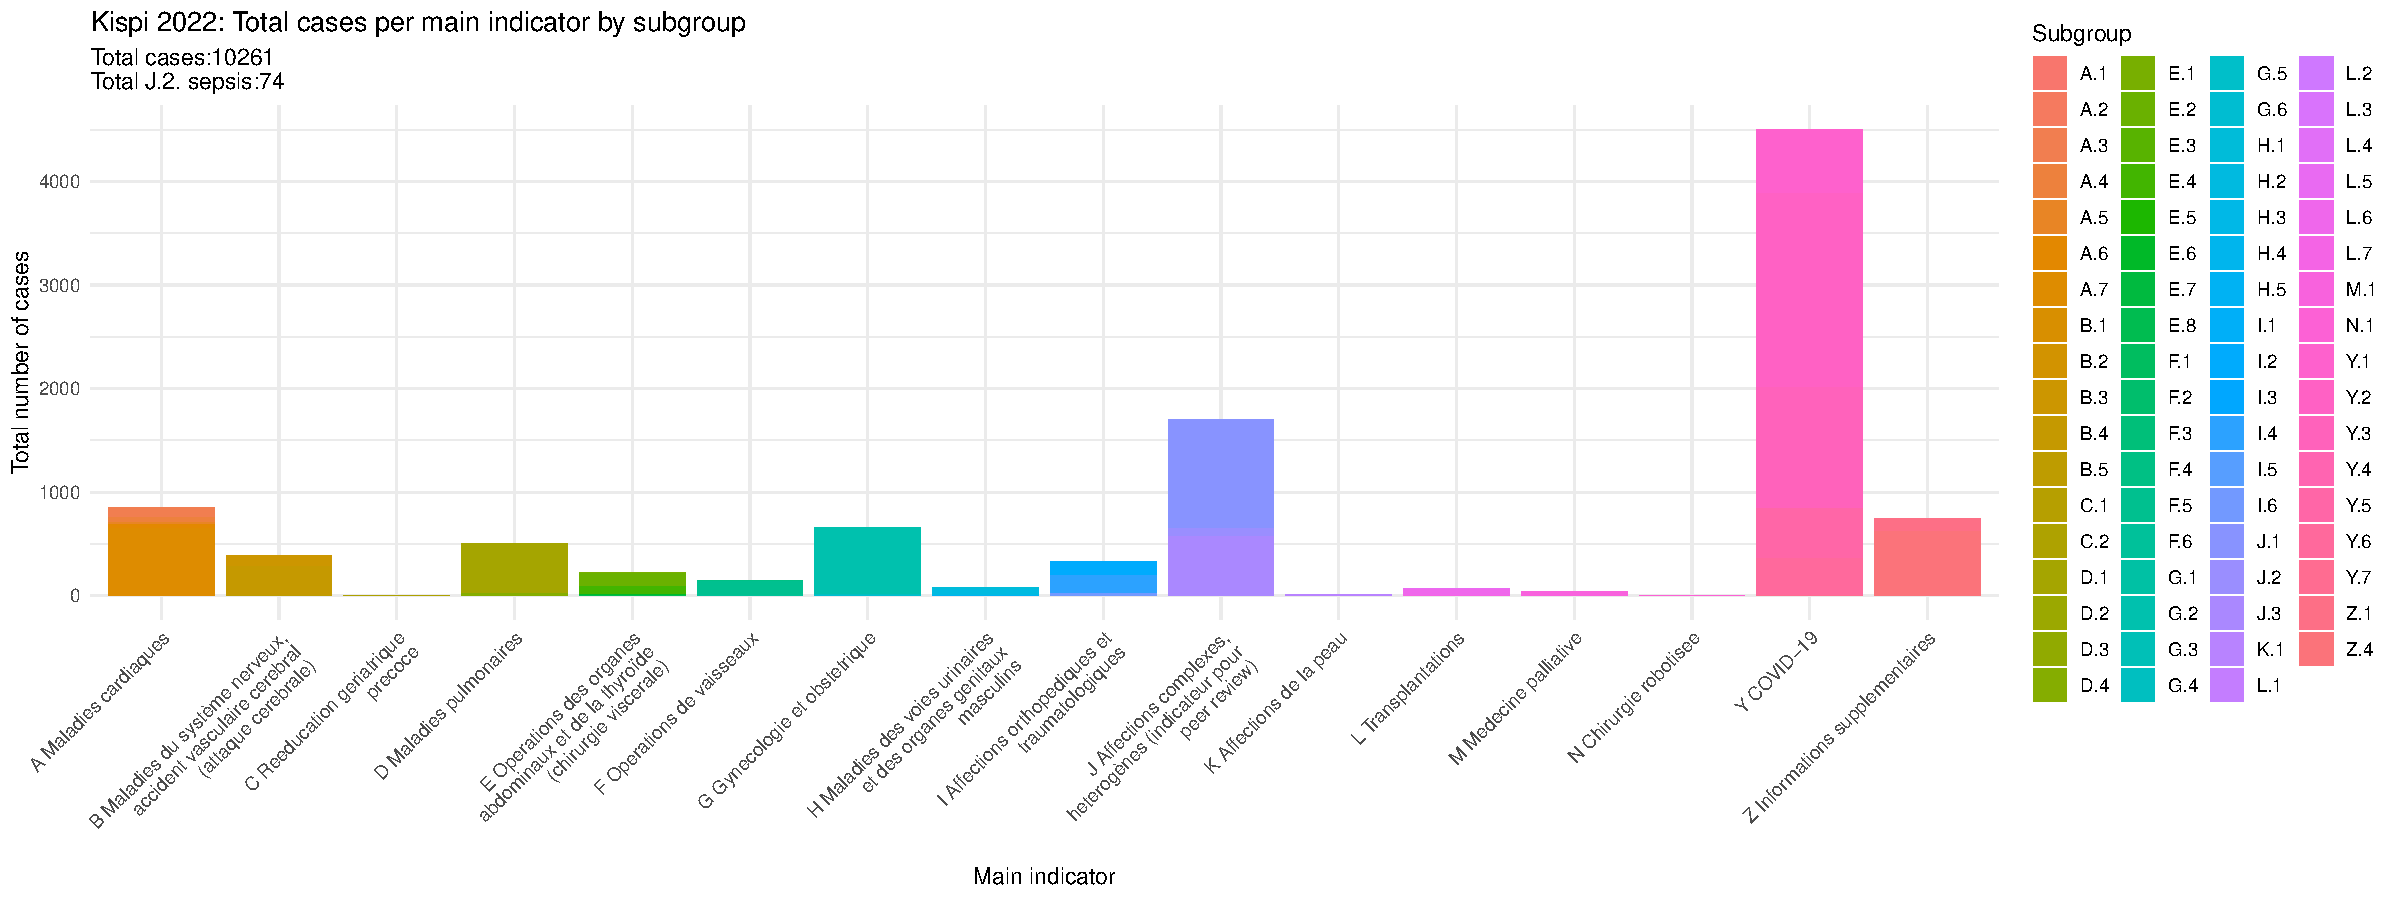
\includegraphics[width=1\textwidth]{../../stats/foph_key_stats/output/p_cases_per_indicator_kispi_2022}
%	\caption{The total count of case descriptions in \kispi for 2022 as categorised according to indicators for the Federal Statistical Office. 
%	The `J.2 Sepsis` subset was used in the other figures shown in this section.}
%	\label{fig:p_cases_per_indicator_kispi_2022}
%\end{center}
%\end{figure}



